% You should title the file with a .tex extension (hw1.tex, for example)
\documentclass[11pt]{article}

\usepackage{amsmath}
\usepackage{amssymb}
\usepackage{fancyhdr}
\usepackage{hyperref}
\usepackage{graphicx}

\oddsidemargin0cm
\topmargin-2cm     %I recommend adding these three lines to increase the 
\textwidth16.5cm   %amount of usable space on the page (and save trees)
\textheight23.5cm  

\newcommand{\question}[2] {\vspace{.25in} \hrule\vspace{0.5em}
\noindent{\bf #1: #2} \vspace{0.5em}
\hrule \vspace{.10in}}
\renewcommand{\part}[1] {\vspace{.10in} {\bf (#1)}}

\newcommand{\myname}{Charles Liu}
\newcommand{\myandrew}{cliu02@g.harvard.edu}
\newcommand{\myhwnum}{2}

\pagestyle{fancyplain}
\lhead{\fancyplain{}{\textbf{HW\myhwnum}}}      % Note the different brackets!
\rhead{\fancyplain{}{\myname\\ \myandrew}}
\chead{\fancyplain{}{CS284}}

\begin{document}

\medskip                        % Skip a "medium" amount of space
                                % (latex determines what medium is)
                                % Also try: \bigskip, \littleskip

\thispagestyle{plain}
\begin{center}                  % Center the following lines
{\Large CS284 Problem Set \myhwnum} \\
\myname \\
\myandrew \\
\today\\
\end{center}

\question{1}{Linear Optimal Control}
\begin{eqnarray*}
	\text{Dynamics: } \dot{x} &=& -2x+5u\\
	\text{Infinite Cost Function: } J &=& \int_{0}^{\infty} (10x^2+u^2)dt
\end{eqnarray*}

\part{a} Given optimal cost-to-go function $J^*=px^2$, we can plug into the HJB equation
\begin{eqnarray*}
	0 &=& min_u[g(x,u) + \frac{\delta J}{\delta x}f(x,u)] \\
	  &=& min_u[10x^2+u^2 + 2px(-2x+5u)] \\
	  &=& min_u[(10-4p)x^2+u^2+10pxu]
\end{eqnarray*}
Finding the minimum, we take $\frac{\delta}{\delta u}$, and find
\begin{eqnarray*}
	2u + 10px &=& 0 \\
	u &=& -5px
\end{eqnarray*}
Substituting back into the HJB equation we get
\begin{eqnarray*}
	0 &=& (10-4p)x^2 + (-5px)^2 + 10px(-5px) \\
	  &=& (10-4p)x^2+25p^2x^2-50p^2x^2 \\
	  &=& (10-4p-25p^2)x^2
\end{eqnarray*}
Since the cost must be positive, $p$ must be the positive root of the quadratic: $\frac{-2+\sqrt{254}}{25}$

\part{b} From part a, $u=-5px=-kx$, meaning $k=5p=\frac{-2+\sqrt{254}}{5}$

\part{c} Changing $g(x,u)$, the equation becomes 
\begin{eqnarray*}
	0 &=& min_u[(20-4p)x^2+2u^2+10pxu]\\
	\frac{\delta}{\delta u} &=& 4u + 10px = 0\\
	u^* &=& \frac{-5px}{2}
\end{eqnarray*}
Substituting back into the HJB equation
\begin{eqnarray}
	0 &=& min_u[(20-4p)x^2+2(\frac{-5px}{2})^2+10px(\frac{-5px}{2})]\\
	  &=& min_u[(20-4p-\frac{25}{2}p^2)x^2]
\end{eqnarray}
The positive root $p = \frac{-4+2\sqrt{254}}{25}$, and $u=-\frac{5px}{2}=-kx$ means $k=\frac{5p}{2}=\frac{-2+\sqrt{254}}{5}$, so (iii) $p$ was doubled

\question{2}{Value Iteration}
\part{a} Recall the analytical solution for the double integrator:
\[
    u= 
\begin{cases}
    1  & \text{if (} \dot{q} < 0 \text{ and } q\leq \frac{1}{2}\dot{q}^2 \text{) or (} \dot{q} \geq 0 \text{ and } q < -\frac{1}{2}\dot{q}^2 \text{)}  \\
    0  & q=0 \text{ and } \dot{q}=0\\
    -1 & \text{otherwise}
\end{cases}
\]
From these equations the boundaries where you can brake to 0 perfectly have deterministic policies, whereas from running the value iteration the policy hovered somewhere in the middle as shown in the graph.\\
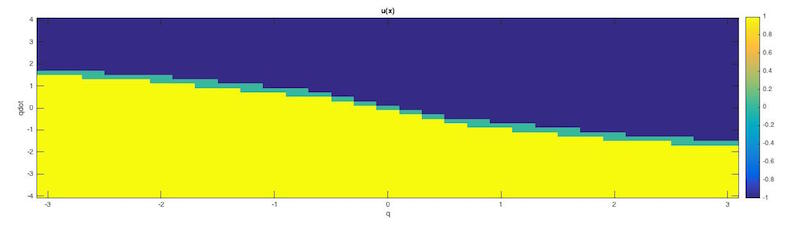
\includegraphics[scale=.6]{dintegrate_valiter}
In particular, in the case where $q(0)=1$, the boundary condition for braking straight to the origin with $u=1$ is when $1 = \frac{1}{2}\dot{q}^2(0)$, meaning $\dot{q}^2(0)=-\sqrt{2}$. However, after returning the MarkovDecisionProcessPolicy object from the DoubleIntegrator code, we see the following:\\\\
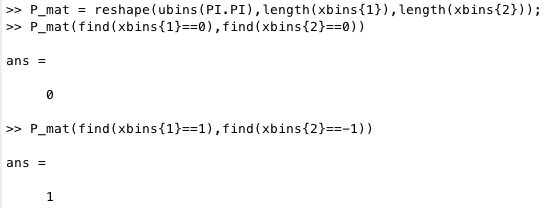
\includegraphics[scale=.75]{doubleint_matlab}\\
The first line formats the policy vector to a matrix, then we see that the origin point returns 0 as expected. The point (1,-1) returns $u=1$ meaning brake, when we know that it should be $u=-1$ (accelerate) until we hit the boundary and then brake.

\part{b} The cost function is 0 if x=[0,0] and 1 otherwise. If xbins doesn't contain the point [0,0] it will never converge. For example, the following initialization of xbins goes from -.1 to .1, skipping 0:\\
\begin{eqnarray*}
xbins = {[-3.1:.2:3.1],[-4.1:.2:4.1]};
\end{eqnarray*}

\question{3}{Acrobot LQR}
\part{a} $u = \pi(A,B,Q,R,K,x,x_0) = -K(x-x_0)$ where $x_0$ is the desired fixed point, in this case the upright position $[[\pi,0],[0,0]]$\\
\part{b} \\
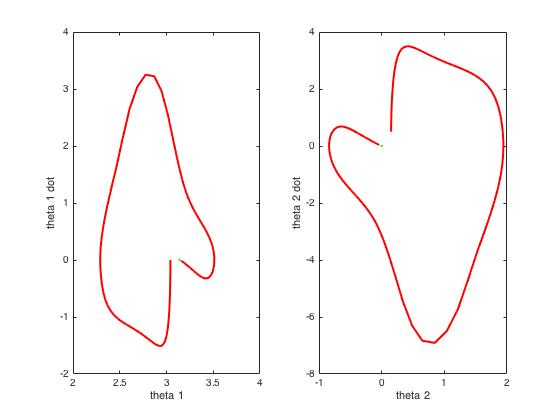
\includegraphics[scale=.6]{3b}

\question{4}{Partial Feedback Linearization}
Equations of motion for Acrobot:
\begin{eqnarray*}
(I_1+I_2+m_2l_1^2+2m_2l_1l_{c2}c_2)\ddot{q}_1\\+(I_2+m_2l_1l_{c2}c_2)\ddot{q}_2-2m_2l_1l_{c2}s_2\dot{q}_1\dot{q}_2-m_2l_1l_{c2}s_2\dot{q}_2^2\\+m_1gl_{c1}s_1+m_2g(l_1s_1+l_{c2}s_{1+2})&=&0\\
(I_2+m_2l_1l_{c2}c_2)\ddot{q}_1+I_2\ddot{q}_2+m_2l_1l_{c2}s_2\dot{q}_1^2+m_2gl_{c2}s_{1+2} &=& \tau
\end{eqnarray*}

Using collocated partial feedback linearization, for some desired $u'$ we set $\ddot{q}_2 = u'$. We then have
\begin{eqnarray*}
\ddot{q}_2 &=& u'\\
-(I_2+m_2l_1l_{c2}c_2)u'+2m_2l_1l_{c2}s_2\dot{q}_1\dot{q}_2+m_2l_1l_{c2}s_2\dot{q}_2^2\\
-m_1gl_{c1}s_1-m_2g(l_1s_1+l_{c2}s_{1+2})\\
------------------------\\
(I_1+I_2+m_2l_1^2+2m_2l_1l_{c2}c_2)&=& \ddot{q}_1
\end{eqnarray*}
To simplify, if
\begin{eqnarray*}
\ddot{q} = \begin{bmatrix} h_1 & h_2 \\ h_2 & h_3 \end{bmatrix}^{-1} (\left[ \begin{array}{c} 0 \\ 1 \end{array} \right]u - \left[ \begin{array}{c} c_1 \\ c_2 \end{array} \right])
\end{eqnarray*}
Then for some $\ddot{q}_2 = u'$
\begin{eqnarray*}
\tau &=& h_2\ddot{q}_1+h_3u' + c_2\\
\ddot{q}_1 &=& \frac{-(h_2u'+c_1)}{h_1}
\end{eqnarray*}

\question{5}{Energy Shaping}
The system's energy eventually oscillates around the desired energy, but the system never reaches the upright configuration as the upper link is in constant motion. $E_{d} - E$ over time:

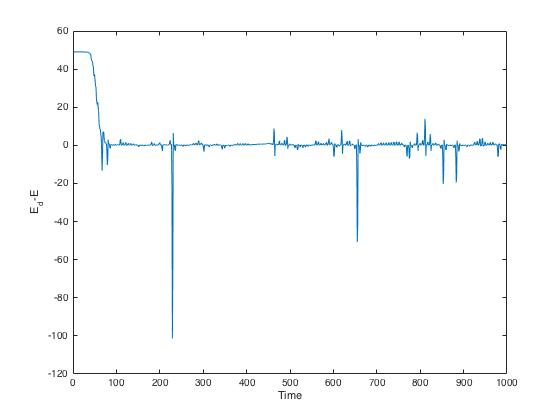
\includegraphics[scale=.75]{E_diff}

\question{6}{Acrobot Swing-up and Balance}
Looks like it has $q_1$ going to $-\pi$ instead of $\pi$ for some reason\\
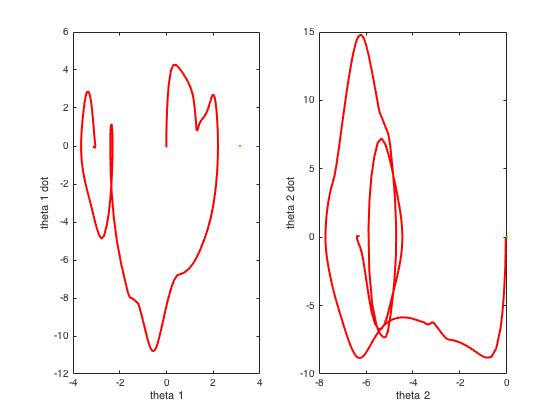
\includegraphics[scale=0.75]{6a.jpg}\\
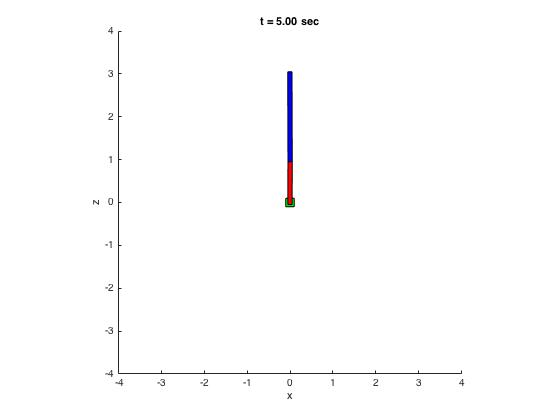
\includegraphics[scale=0.75]{6b.jpg}

\question{7}{Lecture Survey}
(c) Pacing is about right, generally need to review the material after but am understanding concepts.

\question{8}{Pset Survey}
10 hours

\end{document}

